\subsubsection{ClientModel}

\textbf{GoIntentService}

\paragraph{Database}

\textbf{DBHelper}
Die vier nachfolgenden DBHelper erben ihren Konstruktor und ihre Methoden von SQLiteOpenHelper. 
\begin{enumerate}
	\item public DBHelperGroup(context: Context)
		Der Konstruktor definiert dabei den Namen und die Versionsnummer der Datenbank.
	\item public onCreate(sqLiteDatabase: SQLiteDatabase)
		Die SQLiteDatenbank wird mit den in FeedReaderEntry definierten Spalten aufgebaut, wenn sie das erste Mal aufgerufen wird.
	\item public onUpgrade(sqLiteDatabase: SQLiteDatabase, oldVersion: int, newVersion: int)
		Diese Methode wird verwendet, wenn man die Datenbank verändert hat. Dieser wird dann eine neue Versionsnummer zugeteilt.	
\end{enumerate}
\begin{figure}[H]
	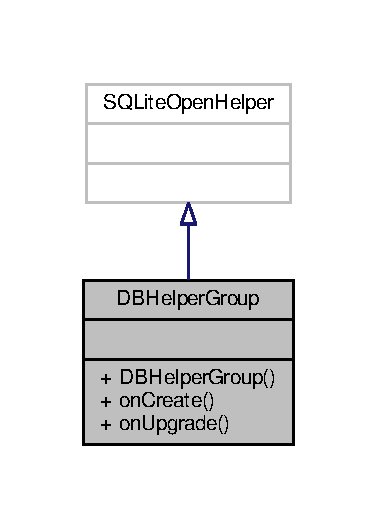
\includegraphics[scale = 1]{res/umlClasses/d_b_helper_group__coll__graph.pdf}
	\centering	
\end{figure}

\begin{figure}[H]
	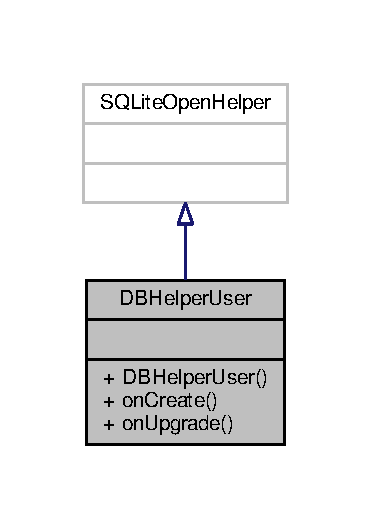
\includegraphics[scale = 1]{res/umlClasses/d_b_helper_user__coll__graph.pdf}
	\centering
\end{figure}

\begin{figure}[H]
	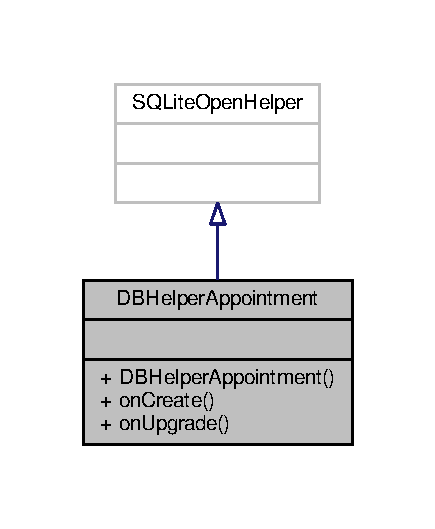
\includegraphics[scale = 1]{res/umlClasses/d_b_helper_appointment__coll__graph.pdf}
	\centering
\end{figure}

\begin{figure}[H]
	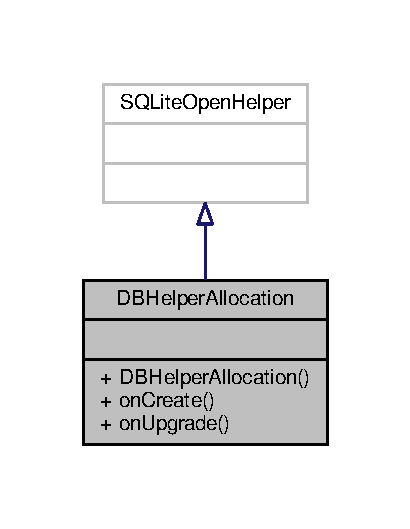
\includegraphics[scale = 1]{res/umlClasses/d_b_helper_allocation__coll__graph.pdf}
	\centering
\end{figure}


\textbf{FeedReaderContract}
\begin{figure}[H]
	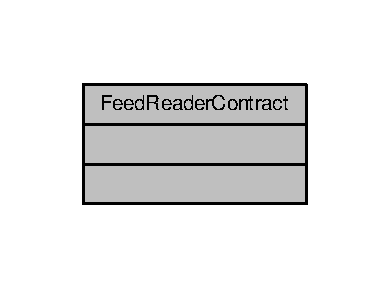
\includegraphics[scale = 1]{res/umlClasses/feed_reader_contract__coll__graph.pdf}
	\centering
\end{figure}
Die FeedReaderContract Klasse definiert in statischen Innenklassen wie die Tabellen der Datenbank aufgebaut sind. Jede der nachfolgenden FeedEntry Klassen implementiert dabei das Interface BaseColumns.

\begin{enumerate}
	\item public static final CREATE ENTRIES:String
		Legt die Spalten wenn die Tabelle generiert wird in genau dieser Reihenfolge an.
	\item public static final DELETE ENTRIES:Strníng
		Löscht die zuvor definierten Spalteneinträge.
\end{enumerate}

\textbf{FeedEntyGroup}
\begin{figure}[H]
	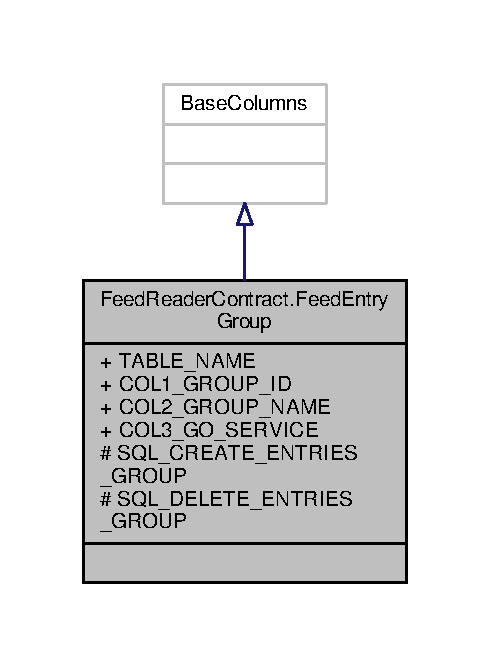
\includegraphics[scale = 1]{res/umlClasses/feed_reader_contract_group.pdf}
	\centering
\end{figure}
Die Innenklasse FeedEntryGroup definiert den Namen und die Spalten der Tabelle, welche die Gruppen auf dem Client speichert. 
Dabei steht in der ersten Spalte die eindeutige Gruppen ID (welche die Zeilen eindeutig unterscheidbar macht), in der zweiten Spalte der eindeutige Gruppenname und in der dritten Spalte, ob der GoService des aktuellen Benutzers für diese Gruppe aktiviert oder deaktiviert ist.
Wenn eine Gruppe gelöscht wird, dann wird auch ihr Eintrag in der Datenbank gelöscht.

\textbf{FeedEntyUser}
\begin{figure}[H]
	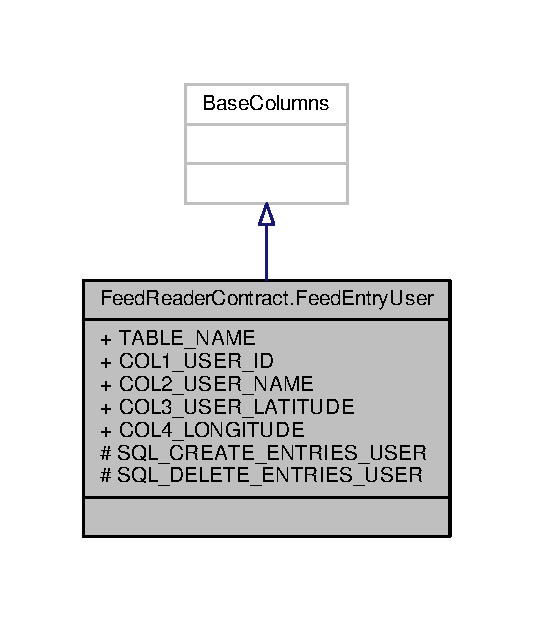
\includegraphics[scale = 1]{res/umlClasses/feed_reader_contract_user.pdf}
	\centering
\end{figure}
Die Innenklasse FeedEntryUser definiert den Namen und die Spalten der Tabelle, welche die Benutzer auf dem Client speichert. 
Dabei steht in der ersten Spalte die eindeutige Benutzer ID (welche die Zeilen eindeutig unterscheidbar macht), in der zweiten Spalte der Benutzername und in der dritten und vierten Spalte steht je ein Wert der zuletzt bekannten Gps Daten des jeweiligen Nutzers. 
Es werden nur Benutzer gespeichert mit denen der aktuelle Benutzer in mindestens einer gemeinsamen Gruppe ist.

\textbf{FeedEntyAppointment}
\begin{figure}[H]
	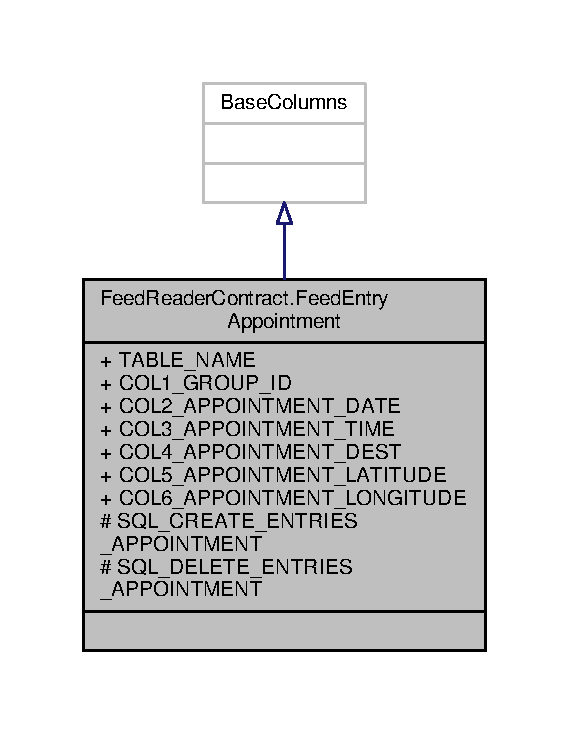
\includegraphics[scale = 1]{res/umlClasses/feed_reader_contract_appointment.pdf}
	\centering
\end{figure}
Die Innenklasse FeedEntryAppointment definiert den Namen und die Spalten der Tabelle, welche die Treffpunkte zu jeder Gruppe speichert. Jede Gruppe hat dabei nur eine Zeile, welche den Treffpunkt definiert. 
Dabei steht in der ersten Spalte die Gruppen id (welche die Zeilen eindeutig unterscheidbar macht), in der zweiten Spalte steht das Datum und in der dritten die Uhrzeit des Treffpunktes. In der vierten Spalte steht der Name des Zielortes und in der fünften und sechsten steht jeweils ein Wert der Gps Daten des Zielortes. 
Wenn sich der Treffpunkt der Gruppe ändert, dann werden die Werte des alten Treffpunktes überschrieben.
Sollte die die Gruppe des dazugehörigen Treffpunktes gelöscht werden, dann wird auch der Eintrag in dieser Tabelle gelöscht.

\textbf{FeedEntyAllocation}
\begin{figure}[H]
	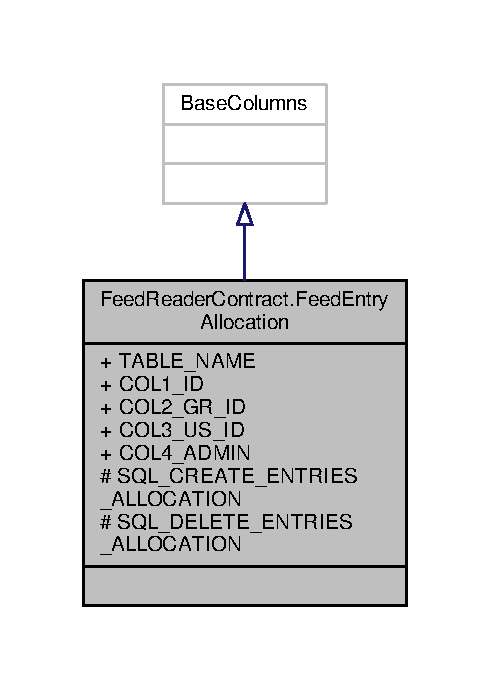
\includegraphics[scale = 1]{res/umlClasses/feed_reader_contract_allocation.pdf}
	\centering
\end{figure}
Die Innenklasse FeedEntryAllocation definiert den Namen und die Spalten der Tabelle, welche die jeweiligen Mitglieder jeder Gruppe speichert, in der der aktuelle Benutzer Mitglied ist. Zu jedem Mitglied wird vermerkt, ob dieses Administratorrechte hat.
Dabei steht in der ersten Spalte die Allocation id (welche die Zeilen eindeutig unterscheidbar macht und automatisch hochgezählt), in der zweiten Spalte steht die Gruppen id, in der dritten Spalte die Benutzer id und in der vierten Spalte, ob dieser Benutzer Gruppenadministrator ist oder nicht. 
Gruppen id wird für jedes Gruppenmitglied vermerkt, also kommt mehrmals vor, sobald mehr als ein Benutzer Mitglied dieser Gruppe ist.


\paragraph{ObjectStructure}

\textbf{GroupClient}
Die Klasse GroupClient definiert wie eine Gruppe auf dem Client aufgebaut ist und welche Funktionalität ihr zur Verfügung steht.
\begin{enumerate}
	\item public GroupClient(name: String, user: UserDecorator)
		Konstruktor der einer neuen Gruppe einen eindeutigen Gruppennamen zuweist und den Ersteller als Gruppenadministrator festlegt.
	\item public createInviteLink():Link
		Um ein Gruppenmitglied hinzuzufügen, muss dieses über einen eindeutigen Link beitreten. Wird der Link ausgeführt wird man entweder zu GoApp weitergeleitet (hat App bereits installiert) oder wird dazu aufgefordert diese zu installieren. Der Link ist nicht mehr gültig sobald das Mitglied hinzugefügt wurde. Man muss Administrator sein um diese Funktion verwenden zu können.
	\item public addGroupMember(user: UserDecorator)
		Ein Mitglied wird der Gruppe hinzugefügt.
	\item public makeGroupMemberToAdmin(user: UserDecorator)
		Ein Gruppenmitglied wird vom Administrator zum Gruppenadministrator gemacht.
	\item public getAllGroupMemberNames():List<String>
		Alle Namen der Mitglieder einer Gruppe werden zurückgegeben.
	\item public deleteGroupMember(user:UserDecorator)
		Ein Gruppenmitglied wird aus der Gruppe durch den Administrator entfernt.
	\item public leaveGroup(user:UserDecorator)
		Ein Mitglied verlässt die Gruppe.
	\item public activateGoService()
		Der aktuelle Benutzer aktiviert seinen GoStatus und übermittelt seine GPS Daten an die Gruppe (GPS muss eingeschalten sein).
	\item public deactivateGoService()
		Der aktuelle Benutzer deaktiviert seinen GoStatus und wird nicht mehr verfolgt.
	\item public changeGroupName(newGroupName:String)
		Der Gruppenadministrator benennt die Gruppe zu einem anderen eindeutigen Namen um.
	\item public getGroupID():int 
		Die Gruppen Id wird zurückgegeben
	\item public getGroupName():String
		Der Gruppenname wird zurückgegeben 
	\item public getGoStatus():GoStatus 
		Der GoStatus wird zurückgegeben
	\item public getAppointment():Appointment 
		Das Appointment wird zurückgegeben
	\item public getMember(userId: int):UserComponent 
		Der Typ des aktuellen Benutzers einer Gruppe (Gruppenmitglied oder Administrator)wird zurückgegeben, um die Ansicht der Gruppe auf seine ihm zugänglichen Funktionen zu beschränken/ erweitern.
\end{enumerate}

\textbf{UserComponent}
Dieses Interface ist die erste Komponente des Decorator pattern und definiert grundlegende Funktionen des Benutzers die jederzeit aufgerufen werden können. 

Mit getUserId() kann der Benutzer von anderen Gruppenmitgliedern unterschieden werden, da der Benutzername nicht eindeutig sein muss, die Id aber schon.
Mit getUserDeviceId() kann der Benutzer auf dem Server angelegt werden. Jede Gerätenummer kann nur einmal auf dem Server vorkommen, um Missbrauch der GoApp vorzubeugen.
\begin{enumerate}
	\item public getUserName():String
	Benutzername des aktuellen Benutzers kann in der GoApp visualisiert werden.
	\item public getUserID():int
	Mit der Benutzer Id kann sich der aktuelle Benutzer unter den anderen Gruppenmitglieder identifizieren.
	\item public getUserDeviceID():String
	Die Device Id wird auf dem Server zusammen mit den anderen zwei Werten gespeichert, um einem Endgerät nur einen Benutzer zu erlauben, um Missbrauch zu vermeiden.
\end{enumerate}

\textbf{SimpleUser}
Die SimpleUser Klasse implementiert das UserComponent Interface. Der Benutzer ist ein SimpleUser Objekt, wenn er nicht in der Gruppenansicht ist und so weder einem Gruppenadministrator noch einem Gruppenmitglied entspricht.
\begin{enumerate}
	\item public getUserName():String
	Siehe UserComponent.
	\item public getUserID():int
	Siehe UserComponent.
	\item public getUserDeviceID():String
	Siehe UserComponent.
	\item public changeUserName(newUserName: String)
	Der aktuelle Benutzer kann seinen Benutzernamen nachträglich ändern.
\end{enumerate}

\textbf{UserDecorator}
Die UserDecorator Klasse ist eine abstrakte Klasse, die wie SimpleUser das UserComponent Interface implementiert. 
Mit getView() kann die Gruppenansicht bestimmt werden indem überprüft wird, ob der Benutzer in der aufgerufenen Gruppe nur Gruppenmitglied oder Administrator ist. Als Administrator stehen dem Benutzer zusätzliche Funktionen zur Verfügung, die dann in der Gruppenansicht angezeigt werden.
Mit getGpsObject() wird die aktuelle Position des Benutzers angefragt, sobald er seinen Go Button aktiviert hat.
\begin{enumerate}
	\item public getUserName():String
	Siehe UserComponent.
	\item public getUserID():int
	Siehe UserComponent.
	\item public getUserDeviceID():String
	Siehe UserComponent.
	\item public getView():boolean
	Mit dieser Methode wird bestimmt welche Gruppenansicht der aktuelle Benutzer sieht (die für ein Gruppenmitglied oder die für einen Gruppenadministrator mit zusätzlichen Funktionen)
	\item public getGpsObject():GpsObject
	Die Gps Daten des aktuellen Benutzers werden zurück gegeben.
\end{enumerate}

\textbf{GroupAdmin}
\begin{enumerate}
	\item
	\item
\end{enumerate}

\textbf{GroupMember}


\textbf{GoStatus}

\textbf{Link}

\textbf{GpsObject}


\textbf{Appointment}

\textbf{AppointmentDate}

\textbf{AppointmentDestination}








